% !TEX program = xelatex
% !TEX encoding = UTF-8
\documentclass{beamer}
\usepackage{ctex, hyperref}

% other packages
\usepackage{amsmath,xcolor,multicol,booktabs,calligra}
\usepackage{graphicx,listings,tikz}
\usepackage{caption}

% sicau beamer
\usepackage{SICAUBeamer}

% 中文字体（无衬线，配合 Beamer 默认风格）
\IfFontExistsTF{Noto Sans CJK SC}{%
  \setCJKmainfont{Noto Sans CJK SC}%
  \setCJKsansfont{Noto Sans CJK SC}%
  \setCJKmonofont{Noto Sans CJK SC}%
}{%
  \IfFontExistsTF{Source Han Sans SC}{%
    \setCJKmainfont{Source Han Sans SC}%
    \setCJKsansfont{Source Han Sans SC}%
    \setCJKmonofont{Source Han Sans SC}%
  }{%
    \setCJKmainfont{Microsoft YaHei}%
    \setCJKsansfont{Microsoft YaHei}%
    \setCJKmonofont{Microsoft YaHei}%
  }%
}

\author[肖宇凌]{作者：肖宇凌}
\title{四川农业大学 Beamer 模板（非官方）}
\subtitle{副标题}
\institute{四川农业大学 \quad xx学院xx专业}
\date{\today}


% defs6
\def\cmd#1{\texttt{\color{red}\footnotesize $\backslash$#1}}
\def\env#1{\texttt{\color{blue}\footnotesize #1}}

\lstset{
    basicstyle=\ttfamily\small,
    keywordstyle=\bfseries\color{red!0!green!0!blue!100},
    emphstyle=\ttfamily\color{red!100!green!0!blue!0},
    stringstyle=\color{red!0!green!100!blue!0},
    numbers=left,
    numberstyle=\small\color{gray!50},
    rulesepcolor=\color{red!20!green!20!blue!20},
    frame=shadowbox
}


\begin{document}
\begin{frame}
    \titlepage
    \begin{figure}[htpb]
       \begin{center}
            
\includegraphics[width=0.2\linewidth]{pic/SIACU_logo.png}
        \end{center}
    \end{figure}
\end{frame}

\begin{frame}
    \tableofcontents[sectionstyle=show,subsectionstyle=show/shaded/hide,subsubsectionstyle=show/shaded/hide]
\end{frame}


\section{课题背景}

\begin{frame}{Why Beamer}
	\begin{itemize}
		\item \LaTeX 广泛用于学术界，期刊会议论文模板
	\end{itemize}
	\begin{table}[h]
		\centering
		\begin{tabular}{cc}
            \toprule
			Microsoft\textsuperscript{\textregistered}  Word & \LaTeX \\
            \midrule
			文字处理工具 & 专业排版软件 \\
			容易上手，简单直观 & 容易上手 \\
			所见即所得 & 所见即所想，所想即所得 \\
			高级功能不易掌握 & 进阶难，但一般用不到 \\
			处理长文档需要丰富经验 & 和短文档处理基本无异 \\
			花费大量时间调格式 & 无需担心格式，专心作者内容 \\
			公式排版差强人意 & 尤其擅长公式排版 \\
			二进制格式，兼容性差 & 文本文件，易读、稳定 \\
			付费商业许可 & 自由免费使用 \\
            \bottomrule
		\end{tabular}
	\end{table}
\end{frame}

\begin{frame}{Why Beamer —— AI 时代的选择}

    {\small\bfseries 核心观点：} 教师专注内容生产，排版与PPT生成交给AI完成。\LaTeX{} 纯文本格式天然适合AI协作。

    \vspace{0.3em}
    \begin{table}[h]
        \centering
        \footnotesize
        \begin{tabular}{p{0.18\paperwidth}p{0.28\paperwidth}p{0.28\paperwidth}}
            \toprule
            \textbf{维度} & \textbf{Word / PPT} & \textbf{\LaTeX{} / Beamer} \\ \midrule
            内容与格式 & 格式内容耦合，调排版耗时 & 样式分离，专注写作 \\
            AI友好度 & 二进制，AI难直接编辑 & 纯文本，AI可直接生成 \\
            版本管理 & 二进制差异难对比 & 文本diff，Git完美支持 \\
            输出一致性 & 不同设备结果不同 & 源码编译，输出一致 \\
            公式与引用 & 排版繁琐，手动维护 & 公式优美，引用自动化 \\
            协作效率 & 多人编辑易冲突 & 文本合并，冲突易解 \\
            \bottomrule
        \end{tabular}
    \end{table}

    \vspace{0.2em}
    {\small\textbf{结论：}AI时代，人负责内容构思，AI负责排版呈现，\LaTeX{} 是最佳人机协作载体。}
\end{frame}



\section{配色说明}

\begin{frame}{配色说明}
    \begin{itemize}
        \item 主色 \textcolor{sicau}{■ RGB(28,108,92)}、浅色 \textcolor{sicauLight}{■ RGB(72,142,128)} 全部取自校徽
        \item 深色 \textcolor{sicauDark}{■ RGB(18,78,64)}、辅助色 \textcolor{sicauVeryLight}{■ RGB(188,210,204)} 用于分层
        \item Logo、水印、标题线、block 颜色保持同一视觉语言
    \end{itemize}
\end{frame}
\section{使用说明}



\begin{frame}[fragile]{\LaTeX{} 常用命令}
    \vspace{-1.2em}
    \begin{table}[h]
        \caption{常用命令}
        \centering
        \footnotesize
        \begin{tabular}{llll}
            \toprule
            \cmd{chapter} & \cmd{section} & \cmd{subsection} & \cmd{paragraph} \\
            章 & 节 & 小节 & 带题头段落 \\ \midrule
            \cmd{centering} & \cmd{emph} & \cmd{verb} & \cmd{url} \\
            居中对齐 & 强调 & 原样输出 & 超链接 \\ \midrule
            \cmd{footnote} & \cmd{item} & \cmd{caption} & \cmd{includegraphics} \\
            脚注 & 列表条目 & 标题 & 插入图片 \\ \midrule
            \cmd{label} & \cmd{cite} & \cmd{ref} \\
            标号 & 引用参考文献 & 引用图表公式等 & \\ \bottomrule
        \end{tabular}
    \end{table}
    \begin{table}[h]
        \caption{常用环境}
        \centering
        \footnotesize
        \begin{tabular}{lll}
            \toprule
            \env{table} & \env{figure} & \env{equation}\\
            表格 & 图片 & 公式 \\\midrule
            \env{itemize} & \env{enumerate} & \env{description}\\
            无编号列表 & 编号列表 & 描述 \\\bottomrule
        \end{tabular}
    \end{table}
\end{frame}

\begin{frame}[fragile]{\LaTeX{} 环境命令举例}
    \begin{minipage}{0.5\linewidth}
\begin{lstlisting}[language=TeX]
\begin{itemize}
  \item A \item B
  \item C
  \begin{itemize}
    \item C-1
  \end{itemize}
\end{itemize}
\end{lstlisting}
    \end{minipage}\hspace{1cm}
    \begin{minipage}{0.3\linewidth}
        \begin{itemize}
            \item A
            \item B
            \item C
            \begin{itemize}
                \item C-1
            \end{itemize}
        \end{itemize}
    \end{minipage}

    \medskip

    \pause
    \begin{minipage}{0.5\linewidth}
\begin{lstlisting}[language=TeX]
\begin{enumerate}
  \item 巨佬 \item 大佬
  \item 萌新
  \begin{itemize}
    \item[n+e] 瑟瑟发抖
  \end{itemize}
\end{enumerate}
\end{lstlisting}
    \end{minipage}\hspace{1cm}
    \begin{minipage}{0.3\linewidth}
        \begin{enumerate}
            \item 巨佬
            \item 大佬
            \item 萌新
            \begin{itemize}
                \item[n+e] 瑟瑟发抖
            \end{itemize}
        \end{enumerate}
    \end{minipage}
\end{frame}

\begin{frame}[fragile]{\LaTeX{} 数学公式}
    \begin{columns}
        \begin{column}{.55\textwidth}
\begin{lstlisting}[language=TeX]
$V = \frac{4}{3}\pi r^3$

\[
  V = \frac{4}{3}\pi r^3
\]

\begin{equation}
  \label{eq:vsphere}
  V = \frac{4}{3}\pi r^3
\end{equation}
\end{lstlisting}
        \end{column}
        \begin{column}{.4\textwidth}
            $V = \frac{4}{3}\pi r^3$
            \[
                V = \frac{4}{3}\pi r^3
            \]
            \begin{equation}
                \label{eq:vsphere}
                V = \frac{4}{3}\pi r^3
            \end{equation}
        \end{column}
    \end{columns}
    \begin{itemize}
        \item 更多内容请自行网上搜索
    \end{itemize}
\end{frame}

\begin{frame}[fragile]{表格与引用}
    \begin{columns}
        \column{.6\textwidth}
\begin{lstlisting}[language=TeX]
\begin{table}[htpb]
  \centering
  \caption{编号与含义}
  \label{tab:number}
  \begin{tabular}{cl}\toprule
  列1 & 列2 \\\midrule
  1 & a\\
  2 & b\\\bottomrule
  \end{tabular}
\end{table}
\normalsize 这里展示引用公式
~(\ref{eq:vsphere})与引用表格
~\ref{tab:number}。
\end{lstlisting}
        \column{.35\textwidth}
        \begin{table}[htpb]
            \centering
            \caption{编号与含义}
            \label{tab:number}
            \begin{tabular}{cl}\toprule
                列1 & 列2 \\\midrule
                1 & a\\
                2 & b\\\bottomrule
            \end{tabular}
        \end{table}
        \normalsize 这里展示引用公式~(\ref{eq:vsphere})与引用表格\ref{tab:number}。
    \end{columns}
\end{frame}
\begin{frame}{建筑物理公式（block示例）}
    \vspace{-0.4em}
    \begin{exampleblock}{围护结构传热}
        \begin{equation*}
            Q = U \cdot A \cdot \Delta T
        \end{equation*}
        其中 $U$ 为传热系数（W/m²K），$A$ 为围护结构面积，$\Delta T$ 为室内外温差
    \end{exampleblock}
\end{frame}


\begin{frame}{场地分析示意（block示例）}
    \begin{columns}[T,onlytextwidth]
        \column{0.48\textwidth}
        \centering
        \begin{tikzpicture}[scale=0.55]
            \fill[sicauVeryLight!40] (0,0) rectangle (8,5);
            \draw[step=1, sicau!20, thin] (0,0) grid (8,5);
            \fill[sicau, opacity=0.15] (2,1) rectangle (6,4);
            \draw[sicau, thick] (2,1) rectangle (6,4);
            \node[sicau] at (4,2.5) {建筑体块};
            \draw[->, sicauDark, thick] (1,4.5) -- (3.5,3.5) node[midway, above, font=\small] {主导风向};
            \fill[blue!40!white] (0.5,3.5) circle (0.3);
            \node[font=\small] at (0.5,3.2) {主入口};
            \draw[sicauLight, dashed] (4,4) -- (4,1);
            \node[sicauLight, font=\small] at (4,4.3) {日照轴};
        \end{tikzpicture}
    \medskip
        
        \small 建筑体块与场地要素关系分析

        \column{0.48\textwidth}
        \begin{exampleblock}{分析要点}
            建筑布局应考虑：
            \begin{itemize}
                \item 日照朝向与建筑间距
                \item 夏季主导风与自然通风
                \item 场地高差与土方平衡
                \item 周边道路与出入口关系
            \end{itemize}
        \end{exampleblock}
    \end{columns}
\end{frame}

\begin{frame}{Nature 风格科学插图}
    \begin{figure}
        \centering
        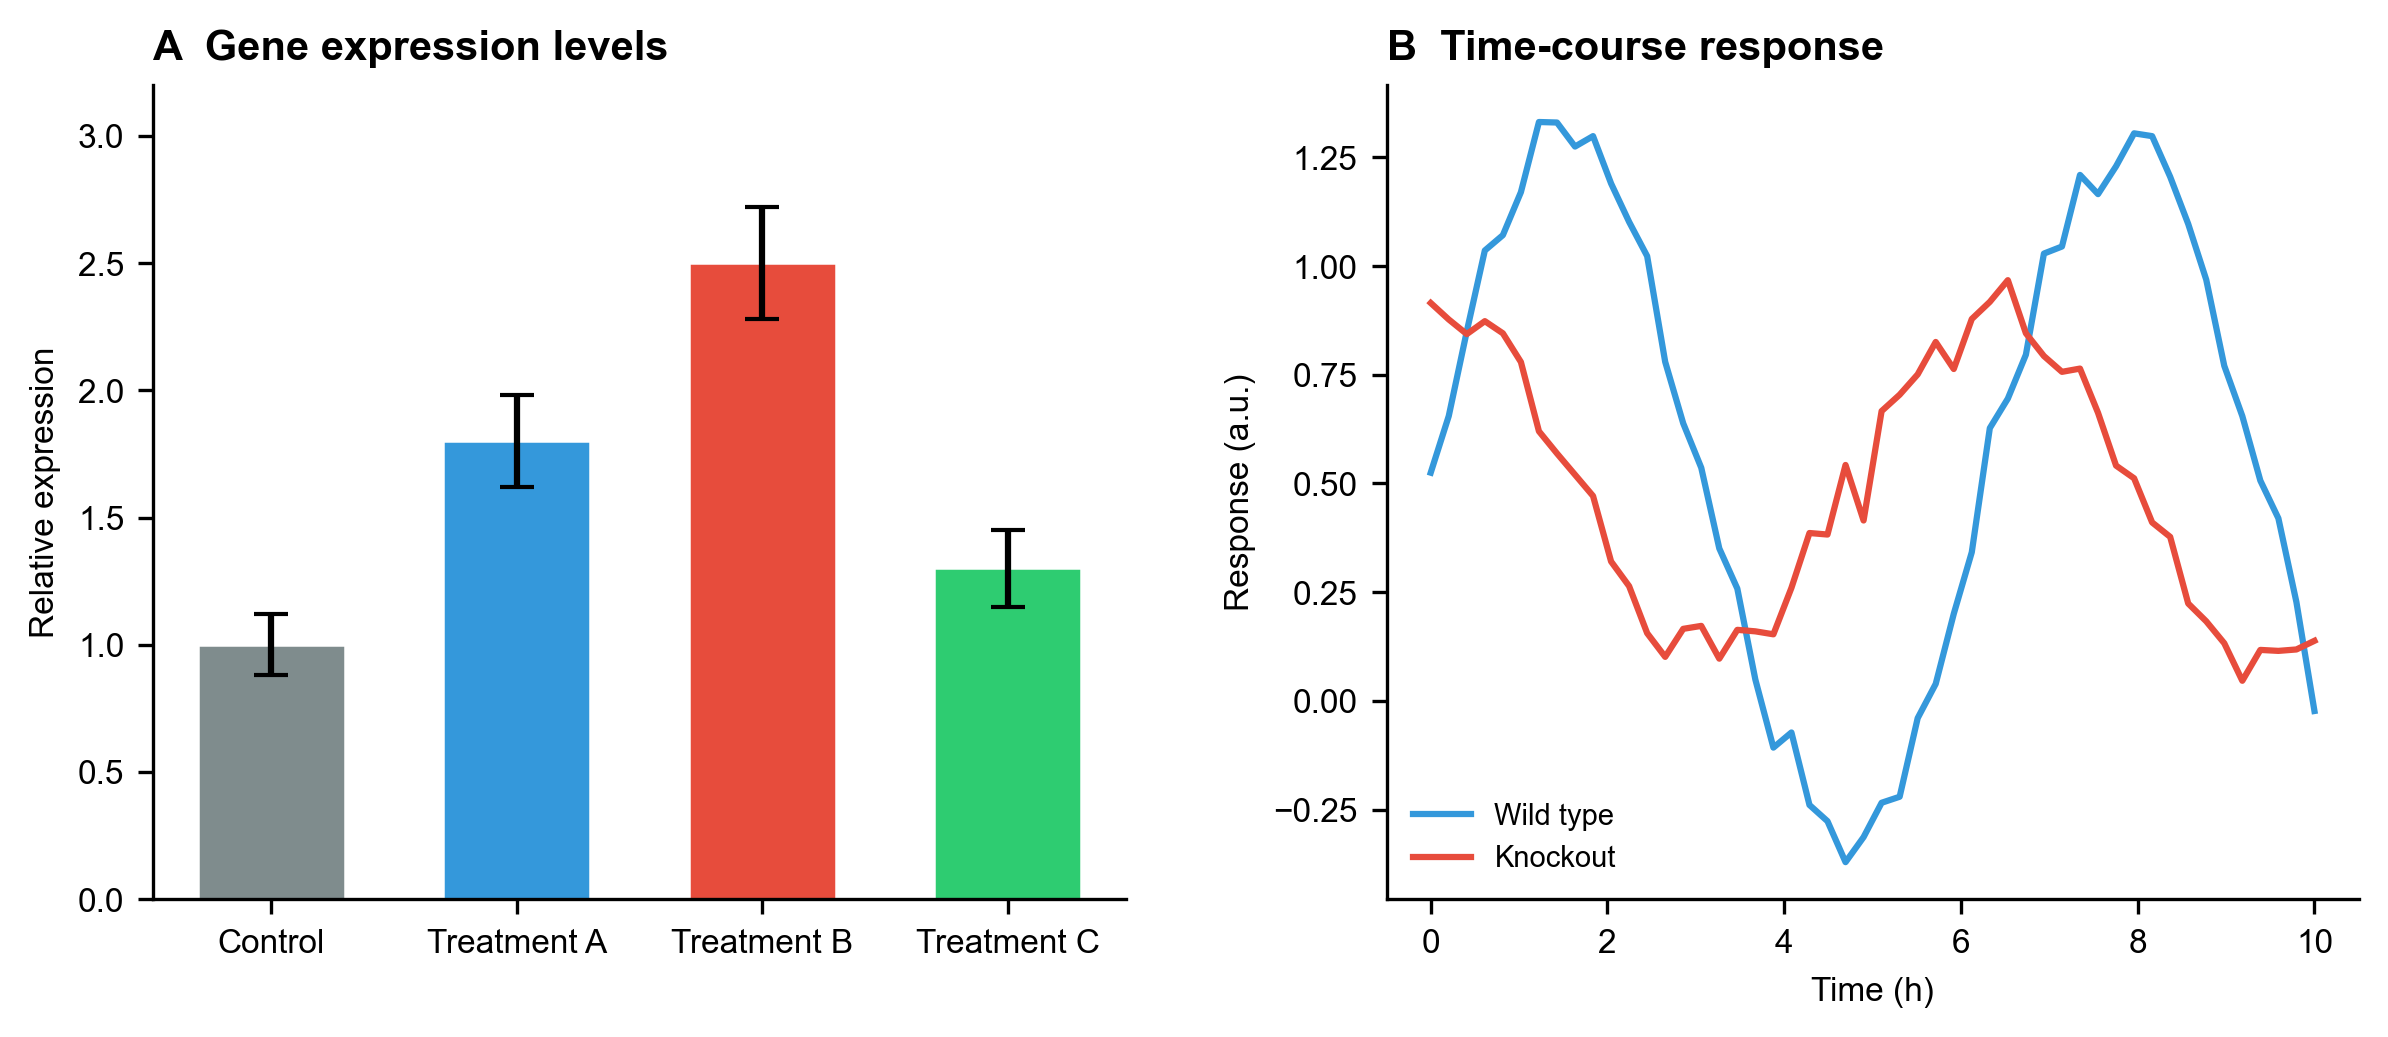
\includegraphics[width=0.85\linewidth]{pic/nature_demo.png}
        \caption{\small 示例双面板图：A 基因表达水平对比；B 时间响应曲线。使用 Python/matplotlib 按照 Nature 期刊风格绘制。}
    \end{figure}
\end{frame}




\section{参考文献}

\begin{frame}[allowframebreaks]
    \bibliography{refe}
    \bibliographystyle{alpha}
\end{frame}

\begin{frame}
    \begin{center}
        {\Huge\calligra Thanks!}
    \end{center}
\end{frame}

\end{document}
